\documentclass[pdftex,a4paper,titlepage,11pt,openright]{article}
\usepackage[T1]{fontenc}
\usepackage[utf8]{inputenc}
\usepackage[english,francais]{babel}
\usepackage{listings}
\usepackage{setspace}

\usepackage{avant}
\usepackage{fancyvrb}
\usepackage{fancyhdr}
\pagestyle{fancy}
\fancyhf{}
\fancyhead[LE,RO]{\itshape\thepage}
% \fancyhead[LO]{\itshape\rightmark}
% \fancyhead[RE]{\itshape\leftmark}
\renewcommand{\headrulewidth}{0.5pt}
\usepackage[top=2.5cm, bottom=2.5cm, left=3.0cm, right=3.0cm, a4paper]{geometry}
% \addtolength{\headheight}{0.5pt}
% \renewcommand\footrulewidth{0pt}
\fancypagestyle{plain}{
    \fancyhead{}
    \renewcommand{\headrulewidth}{0pt}}
\usepackage{textcomp}
\usepackage{relsize}
\usepackage{amssymb}
\usepackage[colorlinks=true,linkcolor=black,citecolor=black,urlcolor=black,filecolor=black]{hyperref}
\usepackage{framed}
\usepackage[pdftex]{graphicx}
\usepackage{makeidx}
% \addtolength{\textwidth}{1cm}
% \setlength{\textheight}{24cm} 	% Hauteur de la zone de texte


% nouvelle commande pour un joli nom
\newcommand{\nom}[1]{\textsc{#1}}

% commande pour une zolie ligne
\newcommand{\ligne}[1][1pt]{
  \par\noindent
  \rule[.5ex]{\linewidth}{#1}\par}

% nettoyer une page blanche avant une page de chapitre en mode openright
\newcommand{\clearemptydoublepage}{
	\newpage{\pagestyle{empty}\cleardoublepage}}


\makeindex

\begin{document}

% augmenter l'espacement entre plusieurs paragraphes plutôt que de passer des lignes quand il faut pas
\setlength{\parskip}{2.4ex}

\title{
\ligne{\Large}
\textbf{Audit Security}\\
\textbf{Project de deuxième année}\\
\Large Généralisation des plugins de communication avec contextd
\ligne{\Large}
}
\author{\nom{Dimitri Gressin} \& \nom{Timothée Ravier}\\\\\nom{Pilote : Jérémy Briffaut}}
\date{17,18,19,20,21 \textsc{janvier} 2011} %TODO

% titre
\maketitle

% page blanche
\clearemptydoublepage

% table des matières
\setcounter{secnumdepth}{2}
\setcounter{tocdepth}{2}
\addtocontents{toc}{\protect\thispagestyle{empty}}
\tableofcontents
\addtocounter{page}{-1}

\newpage

\section*{Introduction} \addcontentsline{toc}{section}{Introduction}
Ce rapport présente le travail et les résultats obtenus à la fin de la première période, dans le cadre de notre projet d'application de deuxième année.
%TODO

~

Le but de ce projet est de remplacer les plugins charger de la communication avec le daemon contextd. En effet, il est pour l'instant nécessaire de modifier chaque application pour lui permettre de valider ses actions avec contextd. L'idée retenue consiste à déplacer la contrainte de communication au niveau du noyau, qui par l'intermédiaire des appels systèmes a connaissance des actions entreprises par les programmes.
%TODO

~

%TODO

~

%TODO

\newpage

\section{Objectifs}

Pour pouvoir se séparer des plugins/modifications par applications, il est nécessaire de communiquer à contextd certaines informations sur le comportement des programmes. Il faut notamment obtenir :
\begin{itemize}
	\item la liste des fichiers créés, ouverts, modifiés par l'ensemble des processus, et les contextes SELinux associés, si le module SELinux est activé.
	\item la liste des connexions ouvertes par le systeme, et plus particulièrement les adresses IP de destination, et donc finalement le nom de domaine de destination.\\
\end{itemize}

De plus, il faut que le programme puisse attendre la réponse de contextd avant de poursuivre sont exécution.

\section{Systemtap}

\subsection{Principe de fonctionnement}

Nous avons ainsi commencer par utiliser Systemtap, un outil d'analyse du noyau grâce à des scripts qui ne nécessite pas de modifier le code du noyau. Systemtap utilise les KProbes, et les Kretprobes\cite{IBMRBST} pour intervenir à différents endroits dans le déroulement des fonctions du noyau pour permettre à l'utilisateur de lire certaines variables, controler... %TODO.

\begin{figure}[hb]
	\centering
	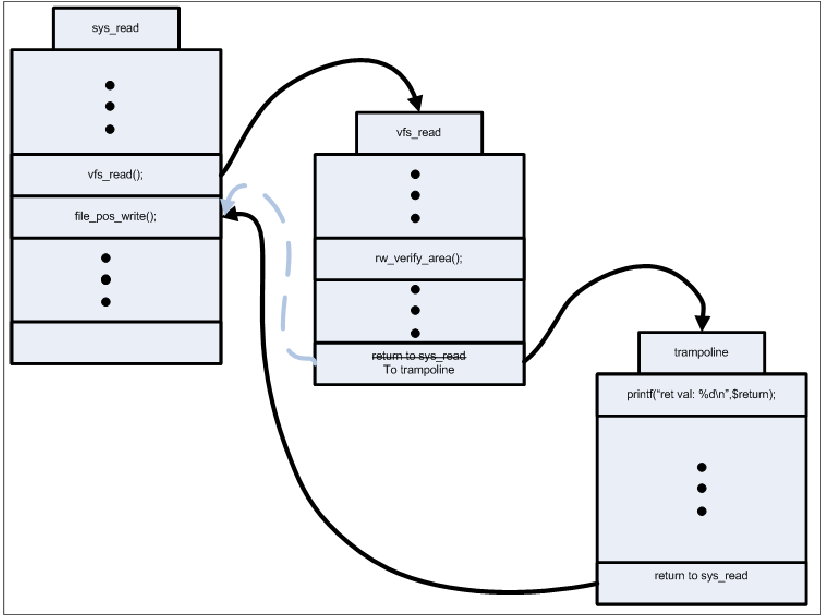
\includegraphics[scale=0.4]{kretprob.png}
	\caption{Fonctionnement tel que décrit dans la référence IBM sur Systemtap \cite{IBMRBST}}
\end{figure}

\subsection{Résultats obtenus}

Nous avons partiellement atteint ces critères mais nous nous sommes rendu compte d'une particularité de l'implémentation de Systemtap qui ne corespondait pas avec notre besoin final. Nous nous sommes heurté à la simplicité de Systemtap qui vise un apprentissage rapide pour un usage ciblé.

De plus, les instructions décrites dans un script écrit pour Systemtap sont exécutées après que le code de l'appel system correspondant ai été exécuté.

%\includegraphics[scale=0.4]{stap_internals.png} TODO

Cela ne correspond donc pas au besoin énoncé précédement.


\newpage


\section{Linux Security Modules}

Nous avons donc décider avec l'accord de Jérémy Briffaut de nous tourner vers les ``Linux Security Modules''.

\subsection{Principe de fonctionnement}

\begin{figure}[hb]
	\centering
	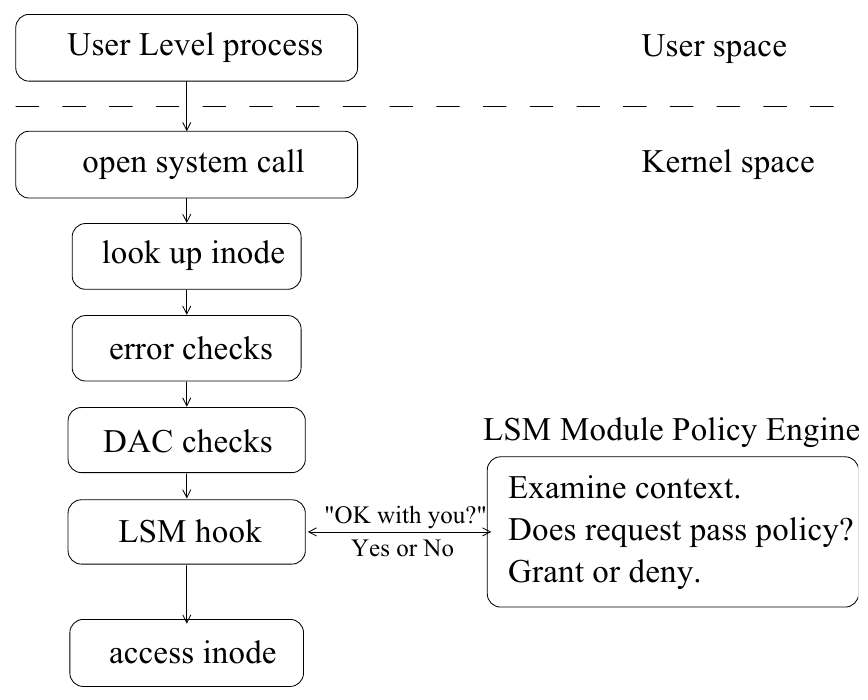
\includegraphics[scale=0.45]{lsm1.png}
	\caption{LSM Hook Architecture \cite{LSMINTRO}}
\end{figure}

\begin{figure}[hb]
	\centering
	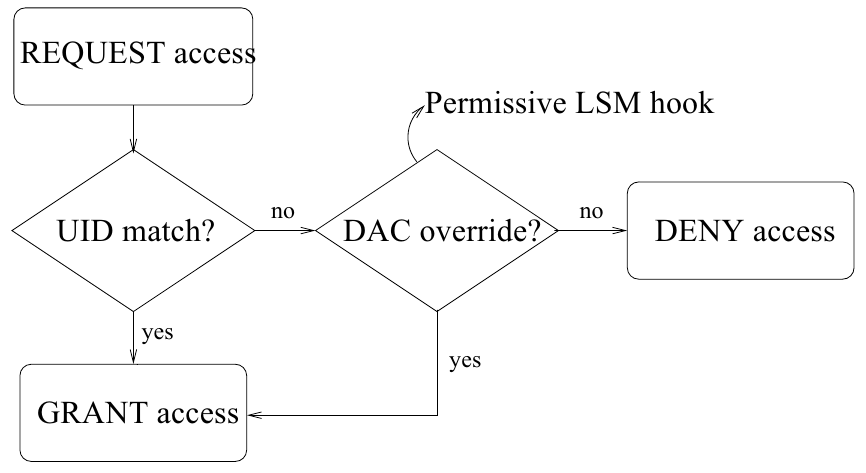
\includegraphics[scale=0.45]{lsm2.png}
	\caption{Permissive LSM hook. This hook allows the security policy to override a DAC restriction \cite{LSMINTRO}}
\end{figure}

\newpage

\subsection{Résultats obtenus}

%TODO

\subsection{Prochain développements}

Création de 3 nouvels appels systèmes pour répondre au besoins de communications entre le noyau et contextd. Pourquoi un appel système plutôt qu'un device ou une fifo? il permet de remplir une structure où nous stockons toutes les informations nécessaires à contextd. Cela nous évite ansi de parser des informations et donc de gagner du temps, resource essentielle vu que chaque appel système ralonge la durée entre la demande d'une application et la réponse finale du noyau.

%TODO Schéma de principe de communication avec le noyau, le daemon, les appels systèmes, contextd.

Pour s'assurer que les communications ne vont pas se mélanger mais bien se dérouler dans l'ordre, nous avons utilisés des verrous au niveau du noyau. Il a donc était nécessaire de vérifier que la mise en place de ces verrous n'entrainait pas d'état bloquant indéfiniement.

% \begin{figure}[hb]
% 	\centering
% 	\includegraphics[scale=0.45]{graphe_verrous.png}
% 	\caption{Graphe des états des verrous au niveau du noyau}
% \end{figure}
%TODO Graphe d'états permettant d'assurer que les verrous dans les appels systèmes n'entrainent pas d'état bloquant sans sortie au niveau du noyau.

\newpage

\clearemptydoublepage

\section*{Conclusion} \addcontentsline{toc}{section}{Conclusion}



Le retard sur la partie implémentation noyau est principalement dûe à notre découverte très progressive des capacités offertes aux développeurs. Le livre Linux Kernel Development \cite{LKDSE} nous a permis de faire un bon en avant et d'implémenter les appels systèmes, ...

%Ce projet aura été pour nous l'occasion d'apprendre un langage de programmation orienté objets, qui nous a permis de gagner en efficacité lors de la phase de développement. En revanche, le fait que nous découvrions le C++ a limité nos possibilités d'optimisations. Le temps de traitement d'un graphe contenant une grande quantité de noeud étant élevé, il paraît nécessaire de paralléliser les algorithmes que nous avons appliqués, pour tirer pleinement partie des machines multi-coeurs ou multi-processeurs, par exemple en utilisant les Intel Threading Building Blocks \cite{IBMRBST}.

%De plus, bien que vérifiée, notre implémentation de l'algorithme de décomposition modulaire peut contenir des bugs. Il faut donc prévoir un outils permettant la vérification des résultats obtenus par cette méthode avec ceux obtenus par le parcours simple de graphes. Il sera donc toujours nécessaire de produire l'intégralité des chemins entre deux noeuds à partir du graphe d'origine pour s'assurer que les graphes réduits sont bien justes.

%Il faut noter, au vu des résultats, que la décomposition modulaire de graphes permettra fort probablement non seulement d'accélerer le parcours de graphes une fois l'intégralité des chemins générés mais aussi de réduire la taille finale de l'ensemble formé par tous les chemins.

%Enfin, notre programme se limite à la décomposition de graphes orientés. Les algorithmes diffèrent de ceux applicables aux graphes non-orientés et leur mise en oeuvre nécessiterai la réécriture d'une grande partie du code pour assurer la rapidité et l'efficacité de notre implémentation.


\newpage
\addcontentsline{toc}{section}{Annexes}
% \addcontentsline{toc}{subsection}{Remarques}
\addcontentsline{toc}{subsection}{Liens et références}
% \subsection*{Remarques}

%Un fichier de configuration est présent avec les sources du kernel 2.6.32-hardened. Il correspond aux options nécessaire à la compilation dans une machine virtuelle Virtualbox. L'option autorisant nos modifications y est aussi activée. Elle est situé dans Security -> SELinux userspace audit.

\subsection*{Liens et références}
\begin{thebibliography}{40}
\bibitem{IBMRBST} \textit{IBM Redbooks : SystemTap: Instrumenting the Linux Kernel for Analyzing Performance and Functional Problems}, \url{http://www.redbooks.ibm.com/abstracts/redp4469.html}

\bibitem{LSMINTRO} \textit{Linux Security Modules : General Security Support for the Linux Kernel}, \url{http://citeseerx.ist.psu.edu/viewdoc/download?doi=10.1.1.84.6867&rep=rep1&type=pdf}

\bibitem{SOURCE} Code source (kernel 2.6.32 hardened r9 et scripts systemtap) disponible sur le serveur de projet STI (le projet s'appelle pour l'instant ``Projet LSM''), \url{http://projetsti.ensi-bourges.fr/projects/promo2012-systemtap}.

\bibitem{LKDSE} \textit{Linux Kernel Development, Second Edition}, Robert Love, Novell Press
\end{thebibliography}

%\printindex

\end{document}
